\usetikzlibrary{decorations.markings,arrows.meta,bending, patterns}

\subsection*{Page 178, Problem 2}
\vspace{15pt}
\begin{proof}
    \vspace{-10pt}
    Given any finite simplicial complex $K$, take any $\alpha \in Z_1(K)$ so $\partial\alpha = 0$ and $\alpha = \sum\limits_{i}c_i (a_i,b_i)$. Note that, by combining like edges (regardless of orientation) and swapping the orientation to flip the coefficent sign, we can rewrite $\alpha$ as $\sum\limits_{i}\lambda_i (u_i, v_i)$ for $\lambda_i \in \Z^+$ and `independent' $(u_i, v_i)$ pairs. Now, $\partial\alpha = 0 \implies \sum\limits_i\lambda_i\partial(u_i,v_i) = \sum\limits_i\lambda_i(v_i-u_i) = 0 \implies \sum\limits_i\lambda_iu_i = \sum\limits_i\lambda_iv_i$. That is the positive integer number of tails at each vertex must also match the number of tips at that vertex.
    
    We can therefore divide $\alpha$ into elementary cycles as follows. Take the edge $1(u_1,v_1)$ in $\alpha$'s linear combination. By our tail-tip argument, there must be some other edge $(v_1, v_i)$ in $\alpha$'s sum for which $v_i \neq u_1$ (else they would have been combined in our earlier simplificiation). We can repeat this process of:
    \[ 
        (u_1, v_1) \overset{v_i \neq u_1}{\longrightarrow} (v_1, v_i) \overset{v_j \neq v_1}{\longrightarrow} (v_i, v_j) \overset{v_k \neq v_i}{\longrightarrow} \cdots \overset{v_m \neq v_l}{\longrightarrow} (v_m, v_n)
    \]
    until the new vertex introduced has already appeared in our sequence. Say we stop here and only take the subsequence from the time it first appeared until the last time, e.g. some 1-cycle $\beta = (v_{\beta_1},v_{\beta_2}) + \cdots + (v_{\beta_n}, v_{\beta_1})$. Because these vertices all originate from our complex $K$ and no vertex appears twice, this is a simple closed polygonal curve. Lastly, $\beta$ has an orientation $(v_{\beta_1}\ldots v_{\beta_n})$ and its boundary vanishes, making $\beta$ an elementary cycle. 
    
    The tail-tip counting argument holds after we subtract $\beta$ from $\alpha$. So, because $\alpha$ is a finite sum, we can repeat this process of discovering new elementary 1-cycles a finite number of times by picking any remaining edge of $\alpha - \beta -  \cdots $ until eventually $\alpha - \beta - \cdots - \gamma = 0$. From this, $\alpha = \beta + \cdots + \gamma$ such that any such element of $Z_1(K)$ is in fact generated by the elementary cycles of $K$. Since all the elementary 1-cycles are also elements of $Z_1(K)$, the elementary 1-cycles exactly generate $Z_1(K)$.
\end{proof}

\newpage
\subsection*{Page 178, Problem 5}
\vspace{15pt}
\begin{proof}
    \vspace{-10pt}
    Take the following triangulation and orientations of the torus $|K|$:
    \begin{center}
        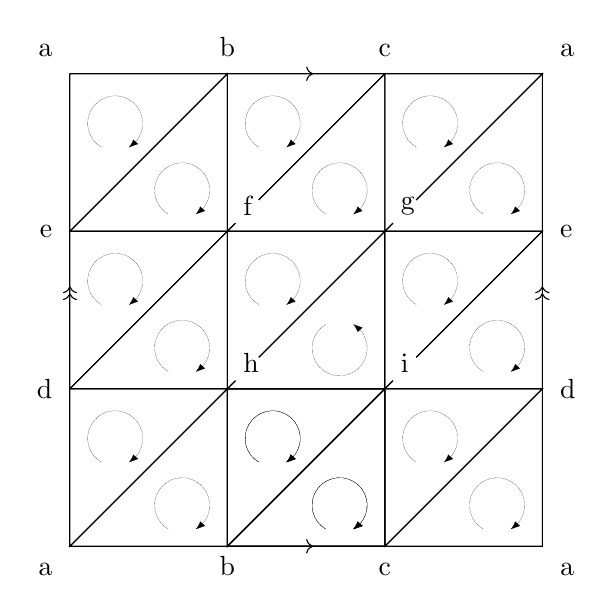
\begin{tikzpicture}
            \tikzset{->-/.style={decoration={
            markings,
            mark=at position #1 with {\arrow{<}}},postaction={decorate}}, ->>-/.style={decoration={
            markings,
            mark=at position #1 with {\arrow{>>}}},postaction={decorate}}}

            \draw[->-=.5] (6,0) node[below right = .1cm]{a} -- (4,0) node[below = .1cm] {c} -- (2,0) node[below] {b} -- (0,0) node[below left = .1cm] {a};
            \draw[->-=.5] (6,6) node[above right = .1cm]{a} -- (4,6) node[above = .1cm] {c} -- (2,6) node[above = .1cm] {b} -- (0,6) node[above left = .1cm] {a};
            \draw[->>-=.55] (0,0) -- (0,2) node[left = .1cm] {d} -- (0,4) node[left = .1cm] {e} -- (0,6);
            \draw[->>-=.55] (6,0) -- (6,2) node[right = .1cm] {d} -- (6,4) node[right = .1cm] {e} -- (6,6);

            \def\boxpath{
                \draw (0,0) -- (2,0) -- (2,2) -- cycle;
                \draw (0,0) -- (0,2) -- (2,2) -- cycle;
                \draw[xshift = 1.5cm, yshift = .65cm, line width=.025pt,-{Latex[bend]}] (240:0.5) arc(240:-60:0.35);
                \draw[xshift = .65cm, yshift = 1.5cm, line width=.025pt,-{Latex[bend]}] (240:0.5) arc(240:-60:0.35);
            }

            \boxpath
            \begin{scope}[xshift = 2cm]\boxpath\end{scope}
            \begin{scope}[xshift = 4cm]\boxpath\end{scope}
            \begin{scope}[yshift = 2cm]\boxpath\end{scope}
            \begin{scope}[xshift = 2cm]\boxpath\end{scope}
            \begin{scope}[xshift = 4cm, yshift = 2cm]\boxpath\end{scope}
            \begin{scope}[yshift = 4cm]\boxpath\end{scope}
            \begin{scope}[xshift = 2cm, yshift = 4cm]\boxpath\end{scope}
            \begin{scope}[xshift = 4cm, yshift = 4cm]\boxpath\end{scope}
            \begin{scope}[xshift = 2cm]\boxpath\end{scope}
            \begin{scope}[xshift = 2cm, yshift = 2cm]
                \draw (0,0) -- (2,0) -- (2,2) -- cycle;
                \draw (0,0) -- (0,2) -- (2,2) -- cycle;
                \draw[xshift = 1.5cm, yshift = 1.25cm, line width=.025pt,-{Latex[bend]}] (240:0.5) arc(-240:60:0.35);
                \draw[xshift = .65cm, yshift = 1.5cm, line width=.025pt,-{Latex[bend]}] (240:0.5) arc(240:-60:0.35);
            \end{scope}

            \draw[white, fill = white] (2.25,2.25) circle (.2cm);
            \draw[white, fill = white] (2.25,4.25) circle (.2cm);
            \draw[white, fill = white] (4.25,2.25) circle (.2cm);
            \draw[white, fill = white] (4.25,4.25) circle (.2cm);
            \draw (2,0) -- (2,2) node[above right = .08cm] {h} -- (2,4) node[above right = .08cm] {f} -- (4,4) node[above right = .08cm] {g} -- (4,2) node[above right = .08cm] {i};
        \end{tikzpicture}
    \end{center}
    Note that all triangles are oriented compatibly except for $\Delta = (ghi)$. That is, all edges are traversed in two opposite ways by certain triangle orientations except for $(ghi)$ which traces its 3 edges in the same direction as its neighboring orientations.

    Consequently, the sum all of these triangles is $K = (abe) + (ebf) + (bcf) + (fcg) + (cag) + (gae) + (def) + (dfh) + (hfg) + (ghi) + (ige) + (ied) + (adh) + (ahb) + (bhi) + (bic) + (cid) + (cda)$. This has boundary $\partial K = \partial (abe) + \cdots + \partial (cda) = ((ab) + (be) - (ae)) + \cdots + ((cd) - (ad) + (ac)) = 2((hi) + (gh) + (ig)) = 2\partial(ghi) = 2\partial\Delta$.
\end{proof}